\documentclass[/home/greg/Thesis/main/main.tex]{subfiles}

%\title{Neutron star mechanics in the observers inertial frame}
%\author{}

\begin{document}
\graphicspath{{/home/greg/Neutron_star_modelling/TimingNoiseModels/Observables_WithTorque/img/}}

\newcommand{\Jr}{\mathbf{J}_{\textrm{rot}}}
\newcommand{\Ji}{\mathbf{J}_{\textrm{in}}}

\section{Biaxial body with torque}

We can now repeat the previous simulations but this time, include the torque.
The torque which produces the observed electromagnetic radiation will play an
important role in determining the time variability of the observed pulse on
earth. The torque is modelled as a magnetic dipole, denoted by $\m$, frozen
into the star at an angle $\chi$ to the $z'$ axis in the $x'-z'$ plane.
Following the work of \citet{Deutsch1955}, the torque is presented here in form
found in \citet{Goldreich1970}.

\begin{equation}
\boldsymbol{T}=\frac{2R}{3c} I_{0}\epsilon_{A}\omega^{2}(\boldsymbol{\omega} \times \hat{\boldsymbol{m}})\times \hat{\boldsymbol{m}} + \epsilon_{A}I_{0}(\boldsymbol{\omega} \cdot \hat{\boldsymbol{m}})(\boldsymbol{\omega} \times \hat{\boldsymbol{m}}), \;\;\;\;\; \textrm{ with } \;\;\;\; \epsilon_{A} = \frac{m^{2}}{I_{0}R_{6}c^{2}},
\label{eqn: torque}
\end{equation}
where $\boldsymbol{\omega}$ is the spin vector and $\epsilon_{A}$ is the magnetic deformation \citep[see][]{Glampedakis2010}.
The first term on the right hand side is often referred to as the \emph{spin down}, or \emph{braking} torque. As this suggests it is responsible for the power law retardation of spin frequency and has an associated timescale $\tau_{S}$. The second term is known as the \emph{anomalous} torque which acts on a timescale $\tau_{A}$. Inserting this torque into the ODEs defined in \eqref{eqn: ODEs} then we have three time scales: the two due to the torque stated above and the precession time scale $\tau_{P}$ as found by \citet{Jones2001}. These three timescales are given by:
\begin{align}
\tau_{P} &= \frac{1}{\epsilon_{I}\nu_{0}}, & \tau_{A}&=\frac{1}{\epsilon_{A}\nu_{0}}, & \tau_{S}&=\frac{3c}{2R}\frac{1}{\epsilon_{A}\nu_{0}^{2}},
\label{eqn: timescales}
\end{align} 
where $\nu_{0}$ is the initial spin frequency and $\epsilon_{I}$ is the magnitude of the elastic deformation along $z$ ($I_{zz} = I_{xx} + \epsilon_{I}$). In previous work we have shown % Maybe include this?
that realistic NSs exist in the region $\tau_{P} > \tau_{A}$ for which $\epsilon_{A} < \epsilon_{I}$, in order to demonstrate the effect of the torque we will work for $\epsilon_{A} = \epsilon_{I}/2$. 
\subsection{Results}
In figure \ref{fig: biaxial body with torque} we plot the spherical components of the spin vector in the body frame (a), and the evolution of the Euler angles. Comparing this with figure \ref{fig: biaxial body no torque} the most striking difference is the wobble in both $\theta$ and $a$, on closer inspection one also finds this wobble in the other angles and the magnitude of $\spin$ along with a monotonic spin down.

\begin{figure}[ht]
	\subfloat[]{\includegraphics[width=0.5\textwidth]{{Spherical_Plot_chi0_8.00e+01_omega0_1.00e+01_epsI3_1.00e-03_n_10000_a0_1.50e+01_T_5.00e+03_upsilon_0.00e+00_epsA_5.00e-04_epsI1_0.00e+00_AnomTorque_1}.pdf}}
	\subfloat[]{\includegraphics[width=0.5\textwidth]{{Euler_Angles_chi0_8.00e+01_omega0_1.00e+01_epsI3_1.00e-03_n_10000_a0_1.50e+01_T_5.00e+03_upsilon_0.00e+00_epsA_5.00e-04_epsI1_0.00e+00_AnomTorque_1}.pdf}}
\caption{Solution to the differential equations in \eqref{eqn: ODEs} including the torque defined in \eqref{eqn: torque} for a biaxial body with $\epsilon_{A}=\epsilon_{I}/2$ }
\label{fig: biaxial body with torque}
\end{figure}•

\FloatBarrier
\subsection{Observables}
In figure \ref{fig: variations with torque} we reproduce plots of figure \ref{fig: variations} with the addition of the torque. The torque introduces two additional effects: $\dot{\Phi}$ the instantaneous electromagnetic frequency decays slowly, this is caused by the spin down torque and is full agreement with what we expect; a fast sinusoidal oscillation in $\dot{\Phi}$ on the spin time scale, observable as a broadening of the line, is a result of the anomalous torque. As for the polar angle $\Theta$ the anomalous torque causes slight changes in the limits of the sinusoidal variation. Both the anomalous torque effects can be understood by realising that this effectively adds a triaxiality into the moment of inertia tensor. % needs more explanation

\begin{figure}[ht]
\centering
	\subfloat[Variations in the spin frequency]{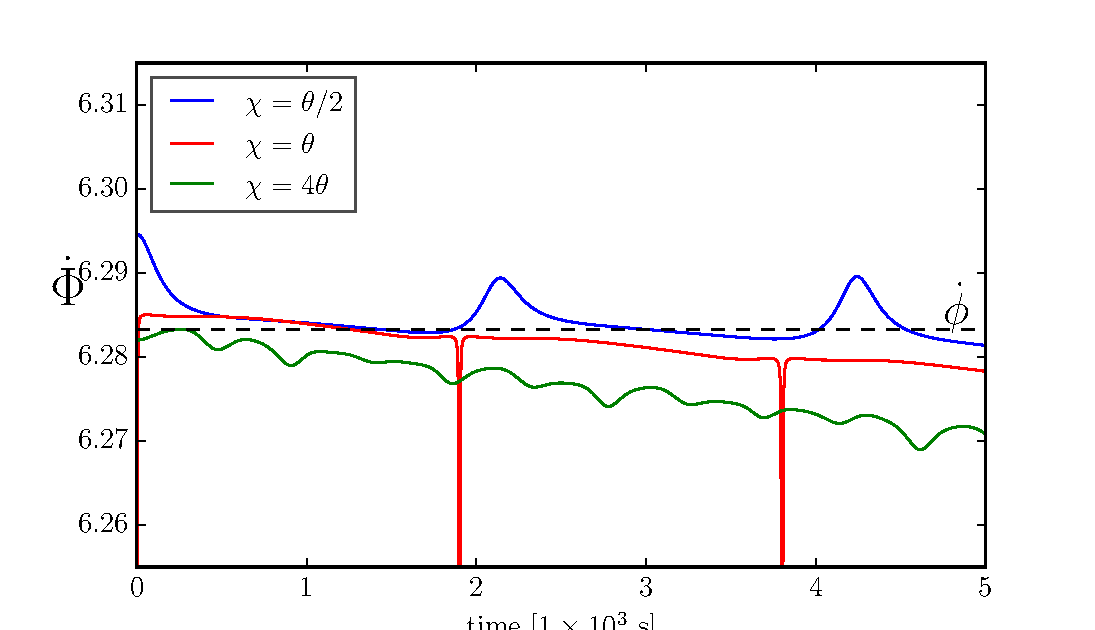
\includegraphics[width=0.7\textwidth]{frequency_variation_with_chi_inc_torque.pdf}} \\
	\subfloat[Variations in polar angle]{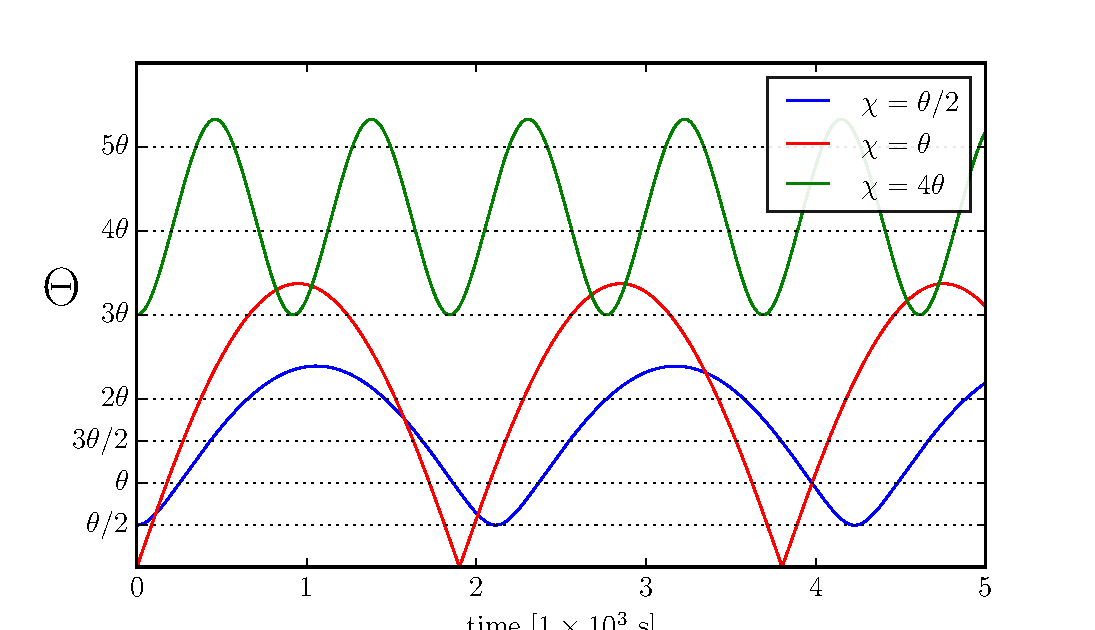
\includegraphics[width=0.7\textwidth]{polar_angle_variation_with_chi_inc_torque.pdf}}
\caption{}
\label{fig: variations with torque}
\end{figure}

\FloatBarrier
\subsubsection{Timing residual}
Including the torque the timing residuals are plotted in figure \ref{fig: TR with torque}, while the sinusoidal variation remains the magnetic inclination varies the spin down rate and hence the period of the these variations.
\begin{figure}[ht]
\centering
	\subfloat[No anomalous torque ]{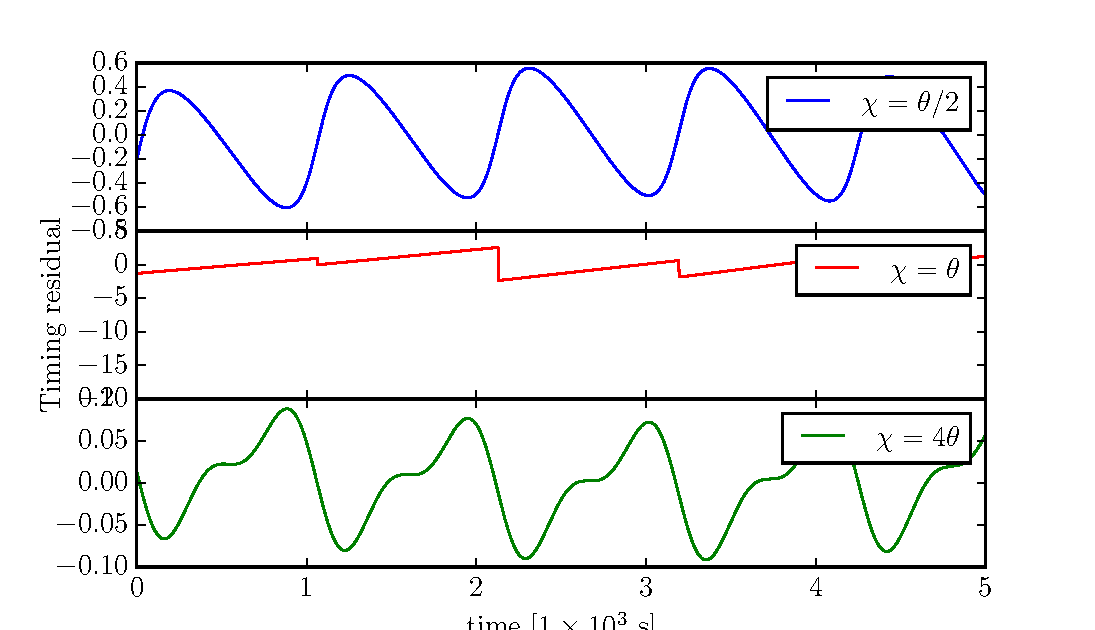
\includegraphics[width=0.6\textwidth]{Timing_residuals_with_torque_no_anom.pdf}} \\
	\subfloat[With anomalous torque]{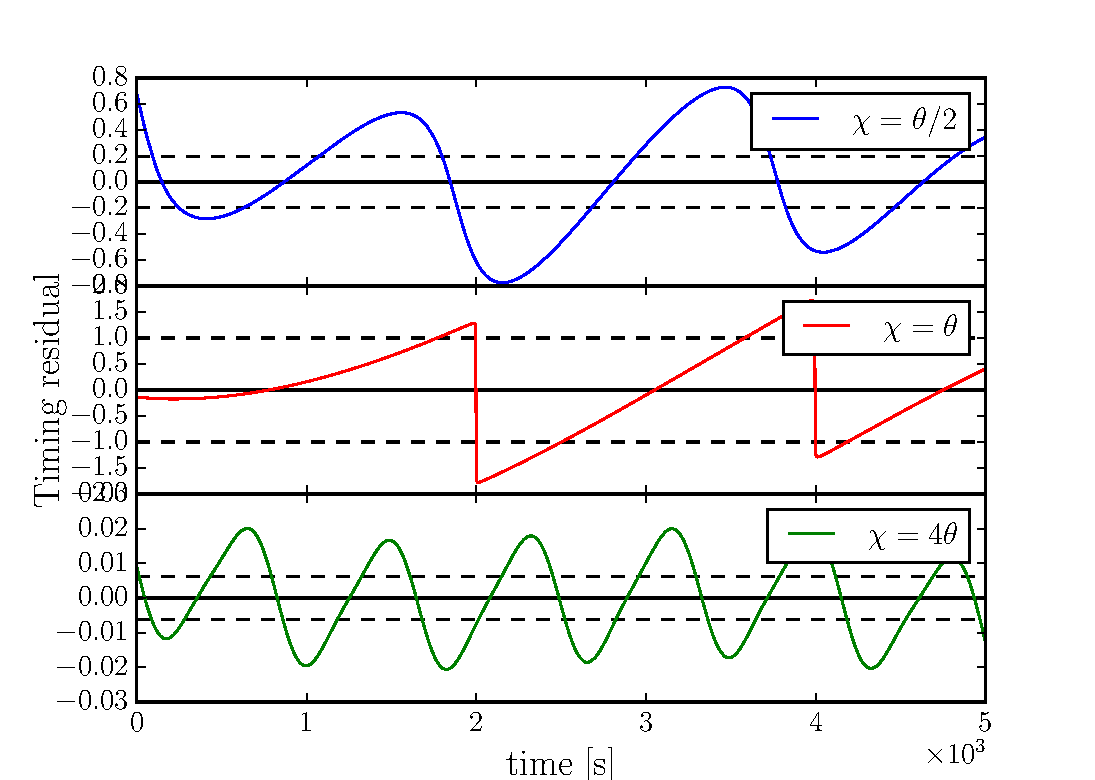
\includegraphics[width=0.6\textwidth]{Timing_residuals_with_torque_with_anom.pdf}}

\caption{Plot of the timing residuals for three angles of $\chi$ including the effects of the torque. }
\label{fig: TR with torque}
\end{figure}

\FloatBarrier
\subsubsection{Spindown Rate $\dot{\nu}$}
The strength of the torque used in this model is parameterised by $\epsilon_{A}$ as given
in equation \eqref{eqn: torque}. From \citet{Shapiro83} we can write this in terms of the
magnetic field strength 
\begin{equation}
B_{s} = \frac{2m}{R^{3}}
\end{equation}•
Considering a simple model of a dipole at an angle $\alpha$ to the spin axis that characteristic
age of NS can be defined as
\begin{equation}
t_{\textrm{ch}} = -\frac{\omega}{\dot{\omega}} = \frac{6 I_{0} c^{3}}{B_{s}^{2}R^{6} \sin(\alpha)^{2}\omega_{0}^{2}}
\end{equation}
Rearranging this expression to solve for the spindown rate yields
\begin{align}
\dot\omega = - \omega \frac{B_{s}^{2}R^{6} \sin(\alpha)^{2}\omega_{0}^{2}}{6I_{0}c^{3}}
\end{align}•
We can write this in terms of the torque deformation
\begin{align}
\dot\omega(t) = - \frac{2}{3}\omega(t) \sin^{2}(\alpha) \omega_{0}^{2} \frac{R}{c}
\label{eqn: EM spindown}
\end{align}

Pulsars, except in rare cases corresponding to globular clusters, have strictly 
negative spindown rates resulting from the electromagnetic torque and 
the emmision of gravitional radiation. To be consistent with observations then
we should constrain outselves to solutions for which the symmetric variations
about the mean spindown as induced by free precession are smaller than the 
spindown given in \eqref{eqn: EM spindown}. From \citet{Jones2001} we can
consider a vacuum point-dipole spin-down torque so that
\begin{equation}
\ddot{\Phi} = k \dot{\Phi} \sin^{2}\Theta
\end{equation}
then departure from a non-precessing power-law spin-down may be written
\begin{align}
\frac{\Delta\ddot{\Phi}}{\ddot{\Phi}} = \left(3 \frac{\Delta\dot{\Phi}}{\dot{\Phi}} + \frac{\Delta(\sin^{2}\Theta)}{\sin^{2}\Theta}\right)
\end{align}
It can be shown that 
\begin{align}
\frac{\Delta\dot{\Phi}}{\dot{\Phi}} & \approx \frac{\cos(\chi)}{\sin(\chi)}\sin(\psi) \epsilon_{I}\theta, &&
\frac{\Delta(\sin^{2}\Theta)}{\sin^{2}\Theta} \approx \frac{2\theta\sin\chi\cos\chi\sin\psi}{\sin^{2}\chi - 2\theta\sin\chi\cos\chi\sin\psi}
\end{align}•

\begin{figure}[ht]
\centering
	\subfloat[No anomalous torque ]{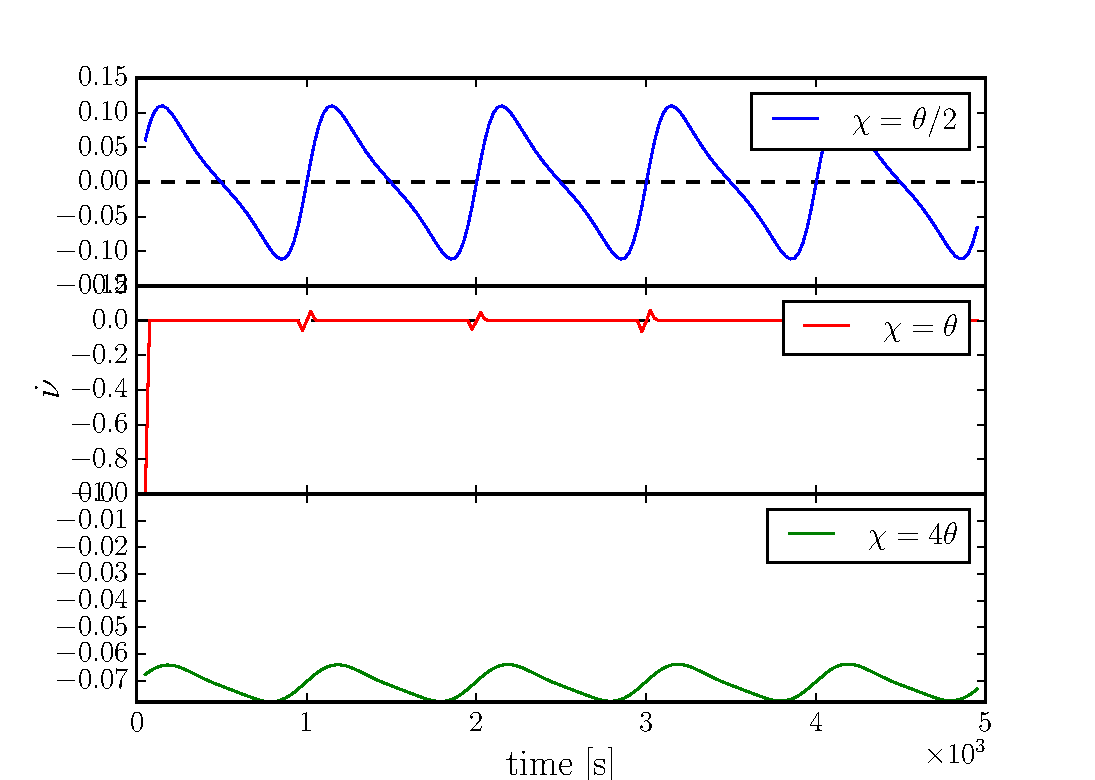
\includegraphics[width=0.6\textwidth]{nu_dot_with_torque_no_anom.pdf}} \\
	\subfloat[With anomalous torque]{\includegraphics[width=0.6\textwidth]{nu_dot_with_torque_with_anom.pdf}}
\caption{}
\label{fig: nu_dot no torque}
\end{figure}

\FloatBarrier

\subsubsection{Pulse amplitude}

\subsubsection{Pulse width}


\FloatBarrier
\section{B1828-11}
In order to compare the prediction of our model with actual observations we select the pulsar B1828-11. There is some evidence in work by \cite{Lyne2000} that this pulsar undergoes precession, and work by \cite{Hobbs2010} and \cite{Lyne2010} documents the timing residuals and spin down rate with unsurpassed accuracy. This makes the pulsar ideal for study under the assumption that the variations are caused by precession.

From table 1 in \citet{Lyne2000} we have that B1828-11 has a spin period of $P_{0}=405$ms. We can calculate the magnetic deformation using the surface magnetic field 
\begin{equation}
\epsilon_{A}=\frac{m^{2}}{I_{0}Rc^{2}}=\frac{(\frac{1}{2}B_{s}R^{3})^{2}}{I_{0}Rc^{2}}
\end{equation}
From table1 we have that $B_{s}=5\times10^{12}$G and using canonical values of $R$, $c$ and $I_{0}$\footnote{Should I give the actual values?} yields $\epsilon_{A}=6.94\times10^{-12}$.

For the elastic deformations we have an upper limit from gravitational wave searches of $1\times10^{-6}$. We now make the assumption that it is precession which causes the variations in signal, from \citet{Jones2001} we may therefore use that 
\begin{equation}
\epsilon_{I} \sim \frac{P_{\textrm{spin}}}{P_{\textrm{precession}}}
\end{equation}•
Lyne found timescales of 1000, 500 and 250 days for the variations, we will use the shortest of these such that $P_{precession}=250$ days. Hence we have an elastic deformations of $1.88 \times10^{-8}$. This also agrees well with \citet{Lyne2010} B1812-11 is observed for $\sim6000$ days during which 22 oscillations occur, this gives a period of about $273$ days. 
With these values we have the following timescales
\begin{equation*}
\tau_{S}=1.06\times10^{15} \textrm{ s} \;\;\;\; \;\;\;\; \tau_{A}=5.83\times10^{10} \textrm{ s} \;\;\;\; \;\;\;\; \tau_{P}=3.55\times10^{6} \textrm{ s}
\end{equation*}•

No obvious way exists to define $\chi$ other than to assume it must not be aligned on grounds that we can observe the pulsar. Since this pulsar satisfies the region A conditions and is therefore subject to the critical of $\chi$ we again choose the two values of $\chi$ previously used.

%\biblio
\end{document}

